% Proposed deployment / graphical abstract: recoater rosette -> inversion -> field.
\documentclass[border=2pt]{standalone}
% ======================================================================
% tikz-common.tex - shared setup for all standalone figures.
% \input this from the preamble of every figures/fig_*.tex.
% ======================================================================

\usepackage{amsmath,bm}
\usepackage{siunitx}
\usepackage{tikz}
\usetikzlibrary{arrows.meta, calc, positioning, patterns, shapes.geometric,
                decorations.pathmorphing, decorations.pathreplacing}
\usepackage{pgfplots}
\pgfplotsset{compat=1.18}
\usepgfplotslibrary{groupplots, colormaps}

% ---- Okabe-Ito colorblind-safe palette --------------------------------
\definecolor{oiBlue}{RGB}{0,114,178}
\definecolor{oiOrange}{RGB}{230,159,0}
\definecolor{oiGreen}{RGB}{0,158,115}
\definecolor{oiVermillion}{RGB}{213,94,0}
\definecolor{oiSky}{RGB}{86,180,233}
\definecolor{oiPurple}{RGB}{204,121,167}
\definecolor{oiYellow}{RGB}{240,228,66}

\pgfplotscreateplotcyclelist{oi}{%
  {oiBlue,       mark=*,         mark size=1.6pt},
  {oiOrange,     mark=square*,   mark size=1.5pt},
  {oiGreen,      mark=triangle*, mark size=1.9pt},
  {oiVermillion, mark=diamond*,  mark size=1.8pt},
  {oiSky,        mark=pentagon*, mark size=1.7pt},
}

% Axis sized for a single column: 76 mm + labels ~ 86 mm total width.
% NOTE: the default legend sits *below* the axis. This is deliberate -- a legend
% inside the axis box routinely lands on top of lines and markers, and judging
% "which corner is free" by eye is unreliable. Parking it outside the data region
% guarantees no overlap. Override per-figure with the named styles below only
% when a corner is provably empty.
\pgfplotsset{
  every axis/.append style={
    width=76mm, height=57mm,
    line width=0.5pt,
    tick style={line width=0.4pt, black},
    grid=major,
    grid style={gray!25, very thin},
    cycle list name=oi,
    legend cell align=left,
    legend style={
      draw=gray!50, fill=white, font=\footnotesize, inner xsep=3pt,
      % default: centered just below the axis, never over the data
      at={(0.5,-0.30)}, anchor=north,
      legend columns=-1,            % single row; use `legend below columns=N' if too wide
      /tikz/every even column/.append style={column sep=6pt},
    },
    label style={font=\small},
    tick label style={font=\footnotesize},
  },
}

% ---- Named legend-placement overrides ---------------------------------
% The default (above) is already overlap-proof. Use these only to relocate the
% legend deliberately; `legend inside' is the ONLY option that risks covering
% data, so reach for it solely when a corner is demonstrably empty.
\pgfplotsset{
  % Stack entries below the axis in N columns (for many series). Usage:
  %   legend below columns=2
  legend below/.style={
    legend style={at={(0.5,-0.30)}, anchor=north, legend columns=-1},
  },
  legend below columns/.style={
    legend style={at={(0.5,-0.30)}, anchor=north, legend columns=#1},
  },
  % Park the legend to the right of the axis (widens the figure ~15 mm).
  legend right/.style={
    legend style={at={(1.02,1)}, anchor=north west, legend columns=1},
  },
  % Opt back IN to a legend inside the axis box. ONLY when the named corner is
  % provably free of lines and markers. Usage: legend inside corner=north east
  legend inside/.style={
    legend style={at={(0.98,0.98)}, anchor=north east, legend columns=1},
  },
  legend inside corner/.style={
    legend style={legend columns=1},
    legend pos=#1,
  },
}

% Backward-compatible alias for the earlier `legend outside' name.
\pgfplotsset{legend outside/.style={legend right}}

% ---- Flowchart / schematic styles --------------------------------------
\tikzset{
  block/.style={draw, rounded corners=2pt, align=center,
                minimum height=2.4em, inner xsep=7pt, inner ysep=4pt},
  decision/.style={draw, diamond, aspect=2.2, align=center, inner sep=1.5pt},
  io/.style={draw, trapezium, trapezium left angle=70,
             trapezium right angle=110, align=center, inner xsep=6pt},
  flow/.style={-{Latex[length=2.2mm]}},
  dim/.style={{Latex[length=1.8mm]}-{Latex[length=1.8mm]}},
}

\begin{document}
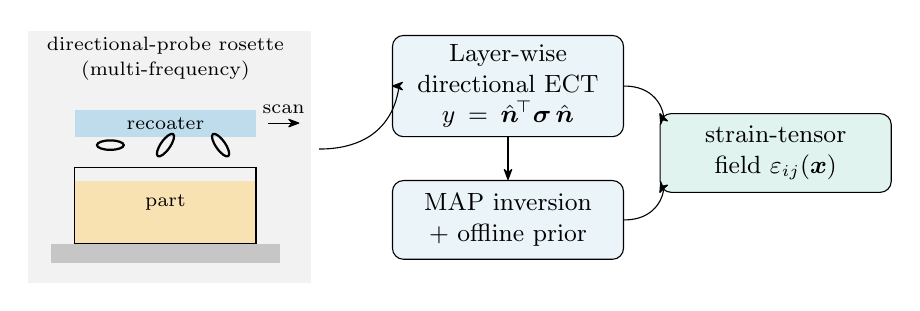
\begin{tikzpicture}[font=\small,
  box/.style={draw, rounded corners, align=center, minimum height=1.0cm,
              text width=2.7cm, fill=oiBlue!8},
  >={Stealth[round]}]
% ---- LPBF machine (left) ----
\fill[gray!10] (-0.1,-0.3) rectangle (3.5,2.9);
\fill[gray!45] (0.2,-0.05) rectangle (3.1,0.2);            % build plate
\foreach \i in {0,1,2,3,4} {
  \fill[oiOrange!30] (0.5,0.2+\i*0.16) rectangle (2.8,0.36+\i*0.16);}
\draw (0.5,0.2) rectangle (2.8,1.16);                       % part
\node at (1.65,0.72) {\scriptsize part};
\fill[oiBlue!25] (0.5,1.55) rectangle (2.8,1.9);            % recoater
\node at (1.65,1.73) {\scriptsize recoater};
\draw[thick] (0.95,1.45) ellipse (0.17 and 0.06);
\draw[thick,rotate around={55:(1.65,1.45)}] (1.65,1.45) ellipse (0.17 and 0.06);
\draw[thick,rotate around={-55:(2.35,1.45)}] (2.35,1.45) ellipse (0.17 and 0.06);
\draw[->] (2.95,1.73) -- (3.35,1.73) node[above,pos=0.5]{\scriptsize scan};
\node[align=center] at (1.65,2.55) {\scriptsize directional-probe rosette\\[-2pt]
  \scriptsize (multi-frequency)};
% ---- workflow (right) ----
\node[box] (ect) at (6.0,2.2) {Layer-wise\\ directional ECT\\
  $y=\hat{\bm n}^{\!\top}\bm\sigma\,\hat{\bm n}$};
\node[box] (inv) at (6.0,0.5) {MAP inversion\\ $+$ offline prior};
\node[box, fill=oiGreen!12] (eps) at (9.4,1.35) {strain-tensor\\ field
  $\varepsilon_{ij}(\bm x)$};
\draw[->] (3.6,1.4) .. controls (4.6,1.4) and (4.6,2.2) .. (ect.west);
\draw[->] (ect) -- (inv);
\draw[->] (inv.east) .. controls (8.0,0.5) and (8.0,1.0) .. (eps.south west);
\draw[->] (ect.east) .. controls (8.0,2.2) and (8.0,1.7) .. (eps.north west);
\end{tikzpicture}
\end{document}
